%Version 2.1 April 2023
% See section 11 of the User Manual for version history
%
%%%%%%%%%%%%%%%%%%%%%%%%%%%%%%%%%%%%%%%%%%%%%%%%%%%%%%%%%%%%%%%%%%%%%%
%%                                                                 %%
%% Please do not use \input{...} to include other tex files.       %%
%% Submit your LaTeX manuscript as one .tex document.              %%
%%                                                                 %%
%% All additional figures and files should be attached             %%
%% separately and not embedded in the \TeX\ document itself.       %%
%%                                                                 %%
%%%%%%%%%%%%%%%%%%%%%%%%%%%%%%%%%%%%%%%%%%%%%%%%%%%%%%%%%%%%%%%%%%%%%

%%\documentclass[referee,sn-basic]{sn-jnl}% referee option is meant for double line spacing

%%=======================================================%%
%% to print line numbers in the margin use lineno option %%
%%=======================================================%%

%%\documentclass[lineno,sn-basic]{sn-jnl}% Basic Springer Nature Reference Style/Chemistry Reference Style

%%======================================================%%
%% to compile with pdflatex/xelatex use pdflatex option %%
%%======================================================%%

%%\documentclass[pdflatex,sn-basic]{sn-jnl}% Basic Springer Nature Reference Style/Chemistry Reference Style


%%Note: the following reference styles support Namedate and Numbered referencing. By default the style follows the most common style. To switch between the options you can add or remove “Numbered” in the optional parenthesis. 
%%The option is available for: sn-basic.bst, sn-vancouver.bst, sn-chicago.bst, sn-mathphys.bst. %  
 
%%\documentclass[sn-nature]{sn-jnl}% Style for submissions to Nature Portfolio journals
%%\documentclass[sn-basic]{sn-jnl}% Basic Springer Nature Reference Style/Chemistry Reference Style
\documentclass[sn-mathphys,Numbered]{sn-jnl}% Math and Physical Sciences Reference Style
%%\documentclass[sn-aps]{sn-jnl}% American Physical Society (APS) Reference Style
%%\documentclass[sn-vancouver,Numbered]{sn-jnl}% Vancouver Reference Style
%%\documentclass[sn-apa]{sn-jnl}% APA Reference Style 
%%\documentclass[sn-chicago]{sn-jnl}% Chicago-based Humanities Reference Style
%%\documentclass[default]{sn-jnl}% Default
%%\documentclass[default,iicol]{sn-jnl}% Default with double column layout

%%%% Standard Packages
%%<additional latex packages if required can be included here>

\usepackage{graphicx}%
\usepackage{multirow}%
\usepackage{amsmath,amssymb,amsfonts}%
\usepackage{amsthm}%
\usepackage{mathrsfs}%
\usepackage[title]{appendix}%
\usepackage{xcolor}%
\usepackage{textcomp}%
\usepackage{manyfoot}%
\usepackage{booktabs}%
\usepackage{algorithm}%

\usepackage{algorithmicx}%
\usepackage{algpseudocode}%
\usepackage{listings}%
\usepackage[
backend=bibtex,
style=alphabetic,
sorting=ynt
]{biblatex}
\addbibresource{sn-bibliography.bib}

%%%%

%%%%%=============================================================================%%%%
%%%%  Remarks: This template is provided to aid authors with the preparation
%%%%  of original research articles intended for submission to journals published 
%%%%  by Springer Nature. The guidance has been prepared in partnership with 
%%%%  production teams to conform to Springer Nature technical requirements. 
%%%%  Editorial and presentation requirements differ among journal portfolios and 
%%%%  research disciplines. You may find sections in this template are irrelevant 
%%%%  to your work and are empowered to omit any such section if allowed by the 
%%%%  journal you intend to submit to. The submission guidelines and policies 
%%%%  of the journal take precedence. A detailed User Manual is available in the 
%%%%  template package for technical guidance.
%%%%%=============================================================================%%%%

%\jyear{2021}%

%% as per the requirement new theorem styles can be included as shown below
\theoremstyle{thmstyleone}%
\newtheorem{theorem}{Theorem}%  meant for continuous numbers
%%\newtheorem{theorem}{Theorem}[section]% meant for sectionwise numbers
%% optional argument [theorem] produces theorem numbering sequence instead of independent numbers for Proposition
\newtheorem{proposition}[theorem]{Proposition}% 
%%\newtheorem{proposition}{Proposition}% to get separate numbers for theorem and proposition etc.

\theoremstyle{thmstyletwo}%
\newtheorem{example}{Example}%
\newtheorem{remark}{Remark}%

\theoremstyle{thmstylethree}%
\newtheorem{definition}{Definition}%

\raggedbottom
%%\unnumbered% uncomment this for unnumbered level heads

\begin{document}

\title[Article Title]{Breast Cancer Image Classification using Convolutional Neural Networks}

%%=============================================================%%
%% Prefix	-> \pfx{Dr}
%% GivenName	-> \fnm{Joergen W.}
%% Particle	-> \spfx{van der} -> surname prefix
%% FamilyName	-> \sur{Ploeg}
%% Suffix	-> \sfx{IV}
%% NatureName	-> \tanm{Poet Laureate} -> Title after name
%% Degrees	-> \dgr{MSc, PhD}
%% \author*[1,2]{\pfx{Dr} \fnm{Joergen W.} \spfx{van der} \sur{Ploeg} \sfx{IV} \tanm{Poet Laureate} 
%%                 \dgr{MSc, PhD}}\email{iauthor@gmail.com}
%%=============================================================%%

\author*[1]{\fnm{Julia} \sur{Graf}}\email{julia.graf@student.uni-tuebingen.de}
\equalcont{These authors contributed equally to this work.}
\author*[1]{\fnm{Jana} \sur{Hoffmann}}\email{jana.hoffmann2@student.uni-tuebingen.de}
\equalcont{These authors contributed equally to this work.}

\author*[1]{\fnm{Jessie} \sur{Midgley}}\email{jessie.midgley@student.uni-tuebingen.de}
\equalcont{These authors contributed equally to this work.}
\author*[1]{\fnm{Maike} \sur{Nägele}}\email{maike.naegele@student.uni-tuebingen.de}
\equalcont{These authors contributed equally to this work.}

\affil*[1]{\orgdiv{Algorithms in Bioinformatics}, \orgname{University of Tübingen}, \orgaddress{\street{Sand 14}, \city{Tübingen}, \postcode{72076}, \country{Germany}}}

%%==================================%%
%% sample for unstructured abstract %%
%%==================================%%

\abstract{Breast cancer, a frequently diagnosed and often life-threatening disease, poses a significant threat, particularly among females. The danger associated with breast cancer underscores the need for advanced techniques to improve the diagnosis of patients suffering from breast cancer. Mammography is a widely used technique for screening breast cancer. In this report, mammographic screens from the CBIS-DDSM Breast Cancer Image Datataset are used to perform binary breast cancer classification into malignant and benign cases. Classification is performed based on a machine learning approach using two different Convolutional Neural Networks (CNNs): VGG16 and ResNet50.Best performance is achieved with the ...  }
%%================================%%
%% Sample for structured abstract %%
%%================================%%

% \abstract{\textbf{Purpose:} The abstract serves both as a general introduction to the topic and as a brief, non-technical summary of the main results and their implications. The abstract must not include subheadings (unless expressly permitted in the journal's Instructions to Authors), equations or citations. As a guide the abstract should not exceed 200 words. Most journals do not set a hard limit however authors are advised to check the author instructions for the journal they are submitting to.
% 
% \textbf{Methods:} The abstract serves both as a general introduction to the topic and as a brief, non-technical summary of the main results and their implications. The abstract must not include subheadings (unless expressly permitted in the journal's Instructions to Authors), equations or citations. As a guide the abstract should not exceed 200 words. Most journals do not set a hard limit however authors are advised to check the author instructions for the journal they are submitting to.
% 
% \textbf{Results:} The abstract serves both as a general introduction to the topic and as a brief, non-technical summary of the main results and their implications. The abstract must not include subheadings (unless expressly permitted in the journal's Instructions to Authors), equations or citations. As a guide the abstract should not exceed 200 words. Most journals do not set a hard limit however authors are advised to check the author instructions for the journal they are submitting to.
% 
% \textbf{Conclusion:} The abstract serves both as a general introduction to the topic and as a brief, non-technical summary of the main results and their implications. The abstract must not include subheadings (unless expressly permitted in the journal's Instructions to Authors), equations or citations. As a guide the abstract should not exceed 200 words. Most journals do not set a hard limit however authors are advised to check the author instructions for the journal they are submitting to.}

\keywords{keyword1, Keyword2, Keyword3, Keyword4}

%%\pacs[JEL Classification]{D8, H51}

%%\pacs[MSC Classification]{35A01, 65L10, 65L12, 65L20, 65L70}

\maketitle

\section{Introduction}\label{Introduction}
Breast cancer is a significant global health concern, impacting the lives of millions each year \cite{siegel2023cancer}. Early detection plays an important role in improving health outcomes and reducing mortality rates in cancer patients \cite{Mathew2018}. Currently, mammograms serve as a primary diagnostic tool in the identification of abnormalities in breast tissue \cite{Mathew2018}. However, the challenge of accurately interpreting these images and distinguishing between cancerous and non-cancerous abnormalities still remains \cite{elter2009}. The use of deep learning methods, particularly Convolutional Neural Networks (CNNs), have had a huge successes in medical image analysis \cite{Cai2020-hn}. Our project centers around the use of CNNs to classify mammograms into benign and malignant cases which, in theory, could aid healthcare professionals in making informed decisions about patient treatment plans. To train our CNNs we made use of the Curated Breast Imaging Subset of the Digital Database for Screening Mammography (CBIS-DDSM) dataset \cite{Lee2017-hi}. Since training a deep CNN requires a sufficiently large dataset in order to avoid overfitting, the issue of limited training samples is often addressed by transfer learning \cite{Kim2022-ge}. This technique uses a larger (often unrelated) database to train an initial model, which can then be fine-tuned on the dataset of interest \cite{Kim2022-ge}. Since large, publicly available medical imaging datasets are limited, we make use of the ImageNet dataset \cite{Deng2009-vj}. To develop our breast cancer classifier, we investigate the performance of two existing CNN architectures, namely VGG-16 \cite{simonyan2015deep} and ResNet-50 \cite{he2015deep}, that have already shown great success for ImageNet classifications, and transfer these pre-learned weights to classify mammogram images. By systematically comparing the performance of these models, we seek to identify the most effective architecture for distinguishing between benign and malignant cases. In addition, we investigate the effectiveness of various image pre-processing and augmentation methods in improving model performance.
 
\section{Materials and Methods}\label{Materials}
\subsection{Dataset}\label{Dataset}
The CBIS-DDSM dataset \cite{Lee2017-hi} is an updated version of the Digital Database for Screening Mammography (DDSM) \cite{Heath2007THEDD}, containing digitized mammograms  in standard DICOM format instead of the, now obsolete, lossless-JPEG format. The subset of 1644 mammography images from 1566 women that are included in the CBIS-DDSM have been selected and curated by a trained mammographer. The dataset is made up of 753 calcification cases and 891 mass cases, with a pathologic diagnosis for each image. We combine these cases and create a random train:test:validation split of 70:20:10.

\subsection{Models}\label{Models}
\subsubsection{ResNet-50}\label{ResNet}
ResNet-50 is a variant of Residual Network (ResNet) architecture, which makes use of skip connections designed to address the vanishing gradient problem. The vanishing gradient problem typically arises during the training of deep neural networks, when the gradients of the loss function become continuously smaller as they are backpropagated through the network. Skip connections allow the gradients  to flow directly though the network, thereby mitigating the vanishing gradient problem. The ResNet-50 architecture consists of 50 layers of weights and several residual learning blocks with varying number of convolutional layers within each block. Each convolutional layer uses Batch normalization as a regularization method. In total, ResNet-50 is made up of a total of  48 convolutional layers, along with 2 pooling layers, producing a grand total of 23 million trainable parameters. The network takes images as input with a dimension of 224 x 224 pixels, and uses softmax in the final layer for the classification of input images \cite{he2015deep}.

\subsubsection{VGG-16}\label{VGG-16}
VGG-16 is a Convolutional Neural Network architecture proposed by Simonyan and Zisserman in 2014, containing 16 layers \cite{Alzubaidi_2021}.
The VGG-16 architecture takes RGB images of a size of 224x224 pixels.\\
The model consists of different types of layers. The early layers in the network comprise 13 convolution layers containing 5 max-pooling layers.
This is followed by 3 dense layers flattening the output of the previous layers and applying a non-linear sigmoid to perform the actual classification. In total, VGG-16 has approximately 15 million trainable parameters \cite{Rahdika_2020}.

\subsection{Hyperparameter}\label{Hyperparameter}
-What hyperparameter settings did you use?
\subsubsection{Preprocessing Images}\label{Preprocessing}
\subsubsection{Fine Tuning}\label{finetuning}
We experiment with re-training the last layer of the pre-trained model with the new images. This means that the original weights from the first to the penultimate layer are preserved or ``frozen", and the last layer is replaced with new weights in order to learn task-specific features. In addition, a final fully-connected layer with 128 units was added to the ResNet-50 model in order to increase the capacity of the model.

\subsubsection{Optimizer and Learning Rate}\label{learningrate}
We compare the performance of two different optimizers, namely Adam and Nadam. Adam computes individual adaptive learning rates for different parameters from estimates of first and second moments of the gradients \cite{kingma2017adam}. Nadam is an extension of the Adam optimizer that incorporates Nesterov momentum and can lead to improved convergence \cite{dozat.2016}.
The learning rate is a hyperparameter of the optimizer, determining the weight with which parameters are updated at each iteration during optimization \cite{Brownlee_2020}.
Yuanyuan et al. even claim that the learning rate is the hyperparameter with the largest influence on the classification accuracy of a model \cite{Yuanyuan_2020}. 
We compare the two optimization algorithms at three different learning rates.
With a larger learning rate, the model tends to converge faster, however with an increased risk of overshooting the optimal value of the loss function \cite{Brownlee_2020}.
If the learning rate is too small, the training process might be time-consuming.
\subsubsection{Flatten vs. Global Average Pooling}\label{fullyConnected}
In order to pass the output of the last convolutional layer to the fully-connected layer and then further to the softmax layer, the vector needs to be converted into a one-dimensional vector. This can be done by applying a flatten layer where the resulting one-dimensional vector contains the same values as before the flattening.\\
Another layer that we can add to reduce the dimensions is a Global Average Pooling layer. This layer creates one feature map for each class of the output and the average of each is passed to the softmax layer \cite{Admin_2023}.
\subsubsection{Image Data Generator}\label{ImageDataGenerator}
For the training we only have 2300 images to train on after splitting the images of the dataset in train, validation and test sets. We compare the performance of our model on these original images in the train set to the images of the train set randomly modified by an ImageDataGenerator from tensorflow before each epoch~\cite{IDG}. We use the following parameters:\\
\begin{itemize}
\item rotation\_range=40
\item width\_shift\_range=0.2
\item height\_shift\_range=0.2
\item shear\_range=0.2
\item zoom\_range=0.2
\item horizontal\_flip=True
\item fill\_mode='nearest'
\end{itemize}
So the input images get randomly flipped by a range between 0° and 40°, shifted on their horizontal axis up to 20\% of their width, shifted on their vertical axis up to 20\% of their height, zoomed by a factor within a range of 0.8 and 1.2, flipped from left to right and the shear transformation is applied to them with an angel of 0.2°. The fill mode fills pixels outside as the nearest pixel. The model than sees more different images. The amount of images that gets seen in each epoch is the same as before.\\
\subsubsection{Data Augmentation}\label{DataAugmentation}
We also test the performance on an augmentation method we wrote ourselves to increase the amount of images the model sees in each epoch. Therefor we implemented the augmentation techniques Montaha et. al. used in their work of the BrestNet18 model~\cite{Montaha2021}. Through the augmentation we generate from each input image of the train set 7 new ones, by flipping vertically, horizontally, vertically and horizontally and rotating the original and the horizontal flipped image by -30° and 30°. After the augmentation the train set includes 18.400 images.\\
\subsubsection{Keeping Height/Width Ratio}\label{HeightWidth}
Since the images in the dataset don't have a height and width of 224 pixels and the models we use have these input dimensions we need to resize the images before we can use them. The build-in function resize from scikit-image doesn't keep the aspect ratio of the pictures it processes~\cite{resize}. Since this can distort important parts of the image we wrote a function that keeps the height/width ratio unchanged while resizing the images. For this we resize the image to the the maximum size in which it still fits in the dimensions (224px,224px) and in which the ratio is kept and fill the parts missing to get a image with the dimensions (224px,224px) black. We compare the performance of the models on images of these two resizing methods.\\




\section{Results}\label{Results}
\subsection{Validation on Best Model}\label{CV_Results}
To evaluate the best VGG16 and ResNet50 model we trained them on 5 different train validation splits and use our pre-defined test set to evaluate the trained model. We generate the different splits by applying the train\_test\_split function from scikit-learn with five times and set the random\_state parameter to None~\cite{TTS}. This way for each run a different values is being used. In the end we plot the ROC-curve for each of these runs and compute the mean test accuracy and the mean test auc.\\


\subsection{VGG-16}\label{VGG-16_Results}
Table \ref{tab1} displays the performance of the model with different hyperparameters. The performance is measured based on two values: the accuracy and the area under the curve (AUC). The first one gives an inside on the correctly predicted classes among all the predictions that have been performed whereas the AUC is based on ... \\
The training of the respective models is performed on a training dataset. Validation is performed on a separate set of images, not seen by the model before.\\
Applying a Global Average Pooling layer instead of a Fatten layer gives rise to worse accuracy and AUC, so does the model, including the self-written preprocessing.\\
The best model is written in bold in the table. The model uses a learning rate of 0.00001, the Adam optimizer, and a flatten layer. The model has a validation accuracy of 72.3\% and an AUC of 80.1\%.\\
Figure \ref{VGG-16_best} shows the training and test accuracy and loss per epoch of the model. Training, as well as validation accuracy, increased whereas the loss decreased. Figure \ref{final-roc} displays the ROC curves for the cross-validation applied to a test set using different train/validation splits. Models 1 and 2 have the highest area under the curve and therefore give the best performance to classify new images. The model achieves a mean accuracy on all splits of 68.6\% and a mean AUC of 73.7\%.


\def\btc{\begin{tabular}{c}}
\def\etc{\end{tabular}}
\begin{table}[h]
\setlength\tabcolsep{4pt}
\caption{Results of VGG-16 hyperparameter tuning}\label{tab1}%
\begin{tabular}{@{}lllllllll@{}}
\toprule
  Prepro & \btc Last Layer\\Trainable \etc  & \btc Adam/ \\ Nadam \etc & \btc Flatten/\\GAP\footnotemark[1]\etc& \btc Learning\\ rate \etc & \btc Data\\ Augm.\footnotemark[2] \etc & \btc H/W \\ Ratio\footnotemark[3] \etc & Acc\footnotemark[4]  & AUC\footnotemark[5]  \\
\midrule
built-in   & yes  & Adam & Flatten  & 0.0001 & no & no & &     \\
built-in   & no  & Adam & Flatten  & 0.0001 & no & no & 0.6933  & 0.7353     \\
self-written   & no  & Adam & Flatten  & 0.0001 & no & no &   0.5920 & 0.6708\\
built-in   & no  & Nadam & Flatten  & 0.0001 & no & no & 0.6656  & 0.7337   \\
\textbf{built-in}   & \textbf{no}  & \textbf{Adam} & \textbf{Flatten}  & \textbf{0.00001} & \textbf{no} & \textbf{no} & \textbf{0.7270}  & \textbf{0.8016} \\
built-in   & no  & Adam & Flatten  & 0.001 & no & no & 0.6748  & 0.7034    \\

built-in  & no  & Adam & GAP  & 0.00001 & no & no &0.5982 & 0.6355    \\
built-in  & no  & Adam & Flatten  & 0.00001 & yes & no &  0.7086  & 0.7487   \\
built-in   & no  & Adam & Flatten & 0.00001 & no & yes & 0.7117  & 0.7286  \\

\botrule
\end{tabular}

\footnotetext[1]{Global Average Pooling}
\footnotetext[2]{using built-in Image Data Generator}
\footnotetext[3]{Keeping height/width ratio}
\footnotetext[4]{Accuracy on validation set}
\footnotetext[5]{AUC on validation set}
\end{table}

\begin{figure}[h]%
\centering
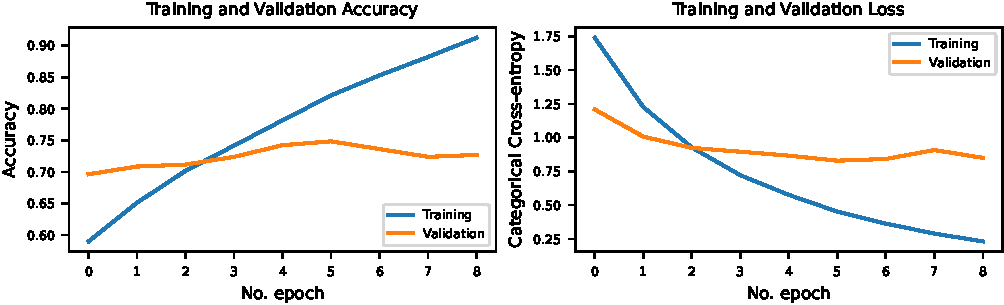
\includegraphics[width=0.9\textwidth]{VGG16_BaseModel-Adam_results_0.00001.pdf}
\caption{Training and validation accuracy and loss of model with best performance }\label{VGG-16_best}
\end{figure}

\begin{figure}[h]%
\centering
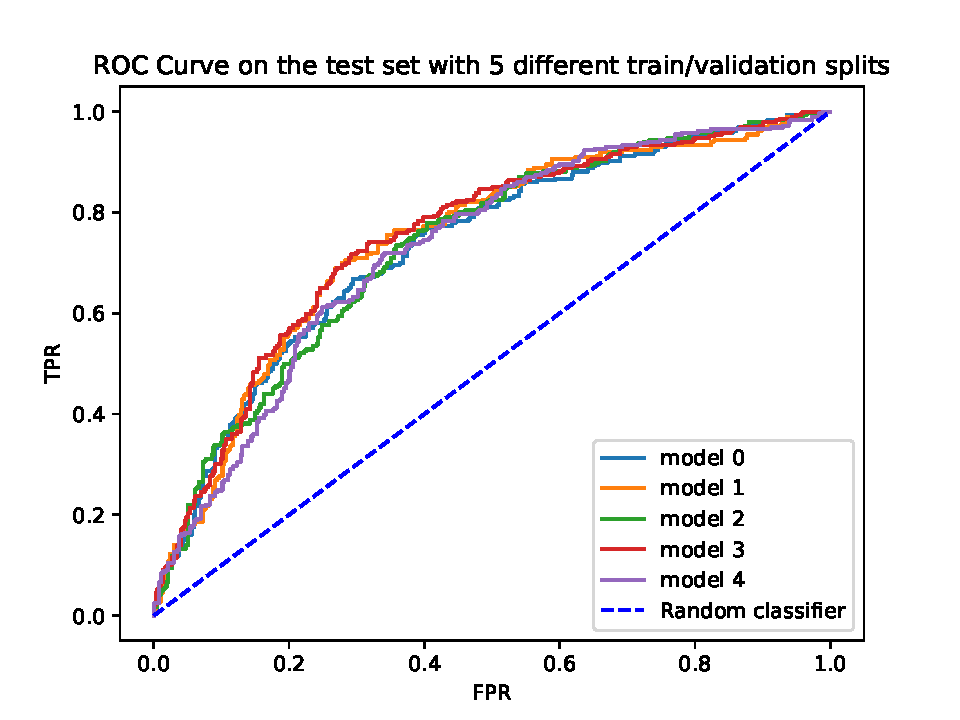
\includegraphics[width=0.6\textwidth]{final_roc.pdf}
\caption{ROC curve after cross-validation of model with best performance using different training/validation splits.}\label{final-roc}
\end{figure}

\subsection{ResNet-50}\label{ResNet_Results}
-- write ResNet results

\def\btc{\begin{tabular}{c}}
\def\etc{\end{tabular}}
\begin{table}[h]
\setlength\tabcolsep{4pt}
\caption{Results of ResNet-50 hyperparameter tuning}\label{tab1}%
\begin{tabular}{@{}lllllllll@{}}
\toprule
  Prepro & \btc Last Layer\\Trainable \etc  & \btc Adam/ \\ Nadam \etc & \btc Flatten/\\GAP\footnotemark[1]\etc& \btc Learning\\ rate \etc & \btc Data\\ Augm.\footnotemark[2] \etc & \btc H/W \\ Ratio\footnotemark[3] \etc & Acc\footnotemark[4]  & AUC\footnotemark[5]  \\
\midrule
built-in   & yes  & Nadam & Flatten  & 0.0001 & no & no & 0.7209  & 0.8036    \\
self-written   & yes  & Nadam & Flatten  & 0.0001 & no & no & 0.6564  & 0.7217 \\
built-in   & no  & Nadam & Flatten  & 0.0001 & no & no & 0.7270  & 0.8234     \\
\textbf{built-in} & \textbf{no}  & \textbf{Nadam}& \textbf{GAP}  & \textbf{0.0001} & \textbf{no} & \textbf{no} & \textbf{0.7515} & \textbf{0.8269}    \\
built-in  & no  & Nadam & GAP  & 0.001 & no & no &  0.7086  & 0.7959   \\
built-in   & no  & Nadam & GAP & 0.00001 & no & no & 0.6871  & 0.7617  \\
built-in   & no  & Nadam & GAP & 0.00001 & yes (self-written) & no & 0.5613  & 0.5914  \\
built-in   & no  & Nadam & GAP & 0.00001 & yes (built-in) & no & 0.6902  &  0.7486 \\
built-in   & no  & Nadam & GAP & 0.00001 & no & yes & 0.6902  &  0.7705 \\

\botrule
\end{tabular}

\footnotetext[1]{Global Average Pooling}
\footnotetext[2]{using built-in Image Data Generator}
\footnotetext[3]{Keeping height/width ratio}
\footnotetext[4]{Accuracy on validation set}
\footnotetext[5]{AUC on validation set}
\end{table}






\section{Discussion}\label{Discussion}
what you did in your project
how you did it
what the results mean?
interpret your results and draw conclusion

\section{Conclusion}\label{conclusion}
In the following report, two existing CNN architectures, namely VGG-16 and ResNet-50 are used to classify mammogram images into benign and malignant.\\
Additionally, data augmentation, data preprocessing, and hyperparamter tuning is performed to achieve better predictions of classes.
Performance analysis of the models indicates the possibilities and benefits of artificial neural networks in health-related issues. \\
For both models an accuracy and AUC of over 65\% is achieved.
Although, the values indicate a moderate performance it is important to consider the limitations for further improvements.
\subsection{Limitations}\label{limitation}
The CBIS-DDSM dataset, used for classification, consists of 1644 images. For a model to perform good classification the size of the available training data plays an important role. As the data is taken from a publicly available source, there is a limited amount of data available. \\
Additionally, the performed classification treats ``benign-without-callback"  and ``benign" identically. However, to ensure correct classification one might have to consider further information for the classification of these images.\\
Finally, hyperparameter tuning was restricted due to time and memory issues. As the servers were not accessible during the time of model training, all the hyperparameter tuning was run locally leading to long runtimes and memory-related issues. 



\printbibliography
\end{document}
